\documentclass{beamer}

\usepackage[british]{babel}
\usepackage{graphicx,hyperref,ru,url}
\usepackage{float}
% The title of the presentation:
%  - first a short version which is visible at the bottom of each slide;
%  - second the full title shown on the title slide;
\title[Brain Racer]{
  Brain Racer}

% Optional: a subtitle to be dispalyed on the title slide

\usepackage{subfigure}
\usepackage[export]{adjustbox}
% The author(s) of the presentation:
%  - again first a short version to be displayed at the bottom;
%  - next the full list of authors, which may include contact information;
\author[Stef, H\'ector, Thomas]{Stef Janssen\\H\'ector van den Boorn\\Thomas van Heyningen }

\begin{document}

\begin{frame}
  \titlepage
\end{frame}

\begin{frame}
  \frametitle{Outline}
  \tableofcontents
\end{frame}

% Section titles are shown in at the top of the slides with the current section 
% highlighted. Note that the number of sections determines the size of the top 
% bar, and hence the university name and logo. If you do not add any sections 
% they will not be visible.


\section{Project}
\begin{frame}
  \frametitle{Problem Description}

  Cybathlon: robust zero training classifier


  \begin{figure}
   
    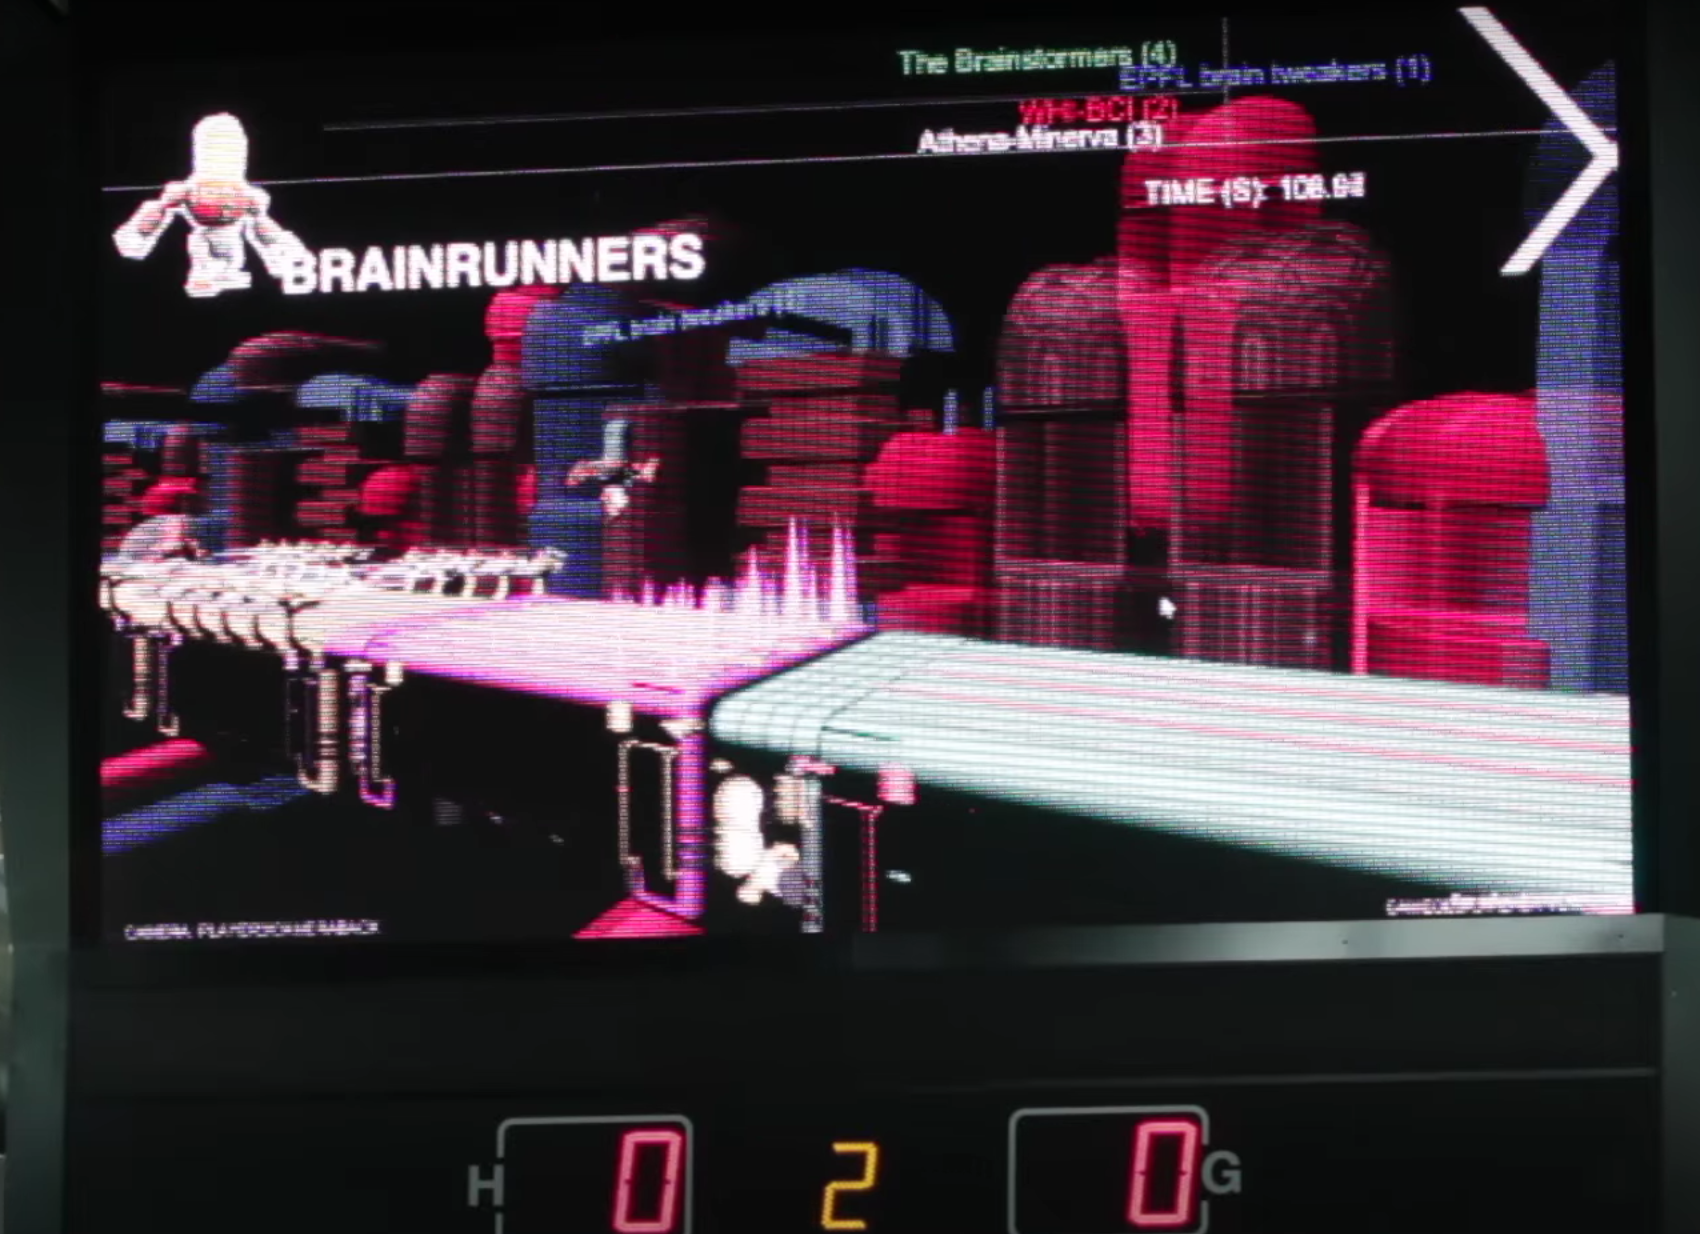
\includegraphics[width=0.5\textwidth]{cybathlon_challenge.png}
  \end{figure}
  
%Ligt toe: simpeler gemaakt naar binaire classificatie
\end{frame}

\begin{frame}
  \frametitle{Foreseen challenges}

  \begin{itemize}
    \item Covariate shift, Bickel et al. 2009
    \item BCI-performance in general
    \item Generalisability between subjects
    \item Online classification
    \item Within subject variation
  \end{itemize}
\end{frame}


\section{Classification scheme}

\begin{frame}
  \frametitle{BCI cycle}
  \begin{figure}
    \centering
    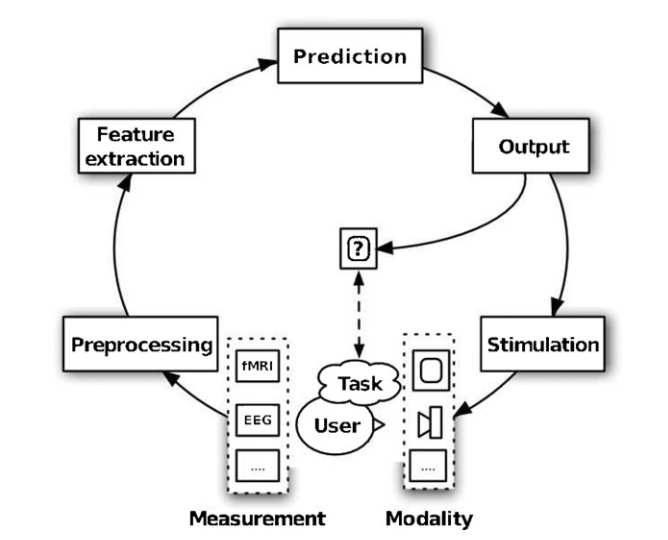
\includegraphics[width=0.7\textwidth]{bci_cycle.png}
  \end{figure}
 
\end{frame}

\begin{frame}
  \frametitle{Preprocessing + Feature Extraction}

  \begin{itemize}
    \item Preprocessing 
	\begin{itemize}
		\item wop
		\item wopwop
	\end{itemize}
    \item Feature Extraction
	\begin{itemize}
		\item wop
		\item wopwop
	\end{itemize}
  \end{itemize}

   

\end{frame}

\begin{frame}
  \frametitle{Prediction}

  \begin{itemize}
    \item List all attempted classifiers
    \item Performance?
  \end{itemize}
\end{frame}

\begin{frame}
  \frametitle{Prediction}

  \begin{itemize}
    \item List all attempted classifiers
    \item Performance?
  \end{itemize}

  \begin{figure}[H]
    
\includegraphics[width=0.3\textwidth, right]{chucktesta.jpeg}
  \end{figure}

\end{frame}

\begin{frame}
  \frametitle{Stimulation}

  \begin{figure}
    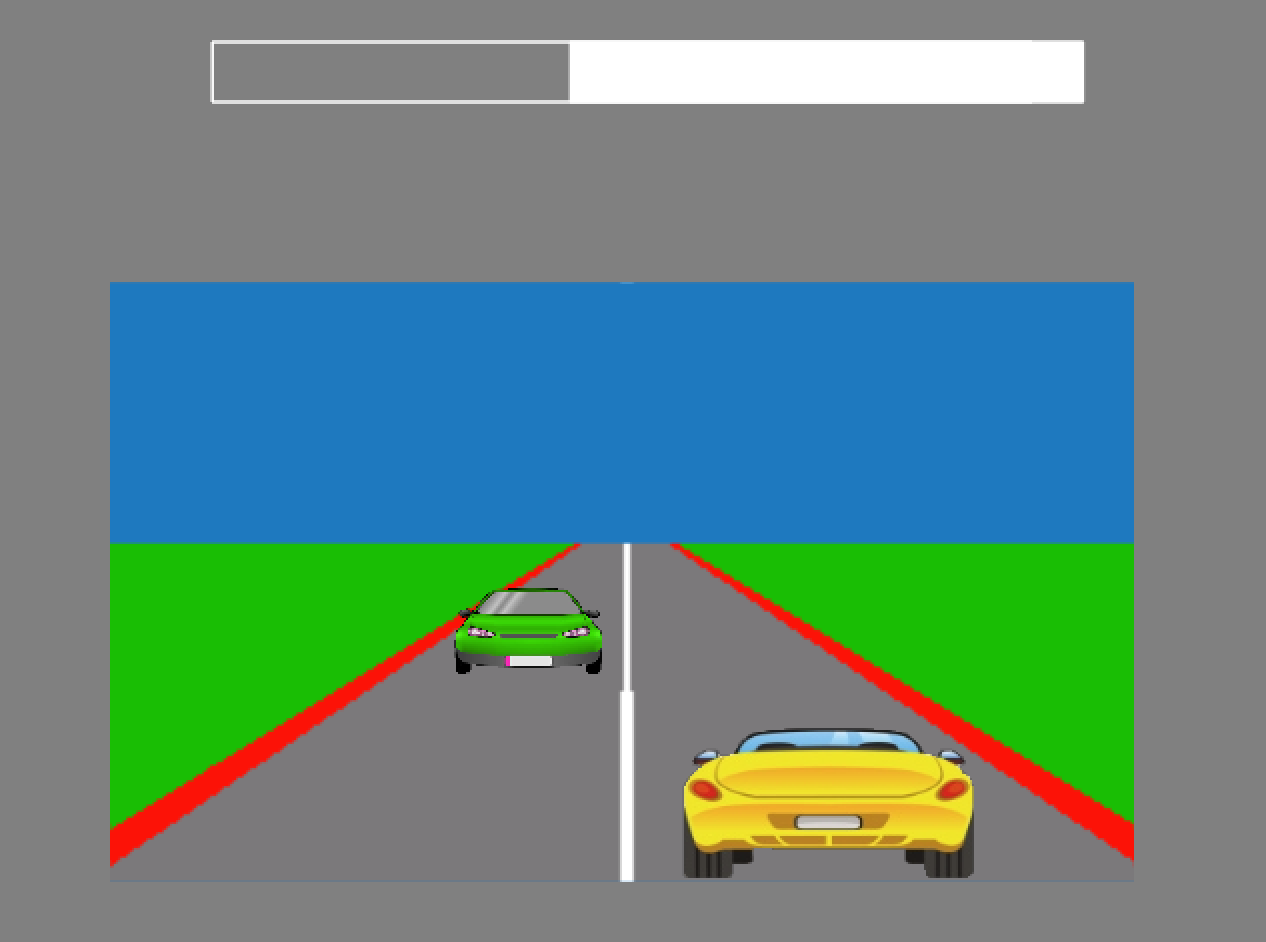
\includegraphics[width=0.7\textwidth]{brain_racer.png}
  \end{figure}

\end{frame}

\section{Experimental setup}

\begin{frame}
  \frametitle{Pipeline}

  \begin{figure}
    \centering
    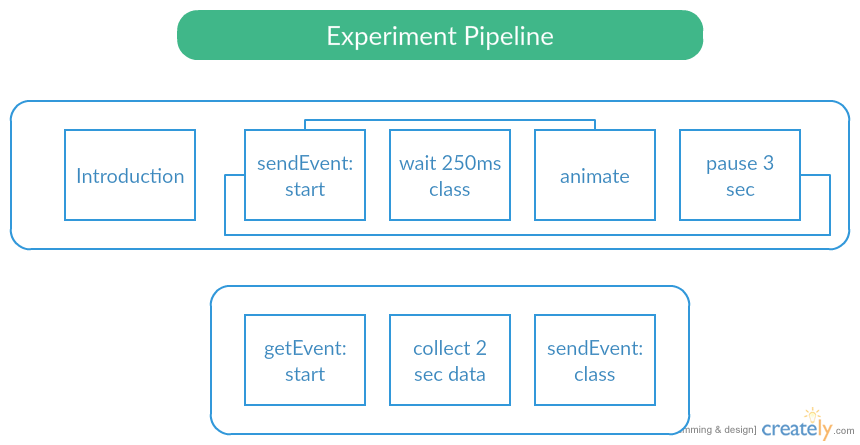
\includegraphics[width=0.9\textwidth]{brain_racer_pipeline.png}
  \end{figure}
\end{frame}


\begin{frame}
  \frametitle{Electrode selection}

 \begin{figure}
  \centering
     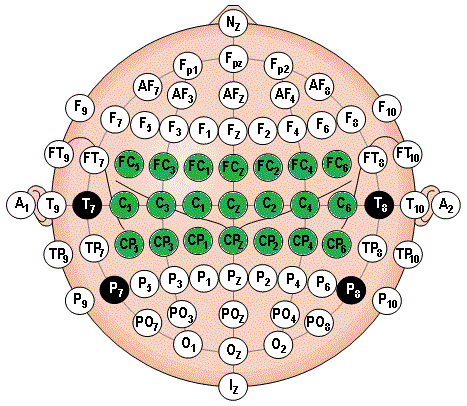
\includegraphics[width=0.7\textwidth]{cap.png}
 \end{figure}

\end{frame}



\section{Results}

\begin{frame}

\frametitle{2 ways of validating}
 \begin{itemize}
   \item Between: Trained on 2 $\rightarrow$ tested on 1
   \item Within: Cross validated on each subject
 \end{itemize}

\end{frame}

\begin{frame}
  \frametitle{WOPWOP}

 \begin{figure}
  \centering
     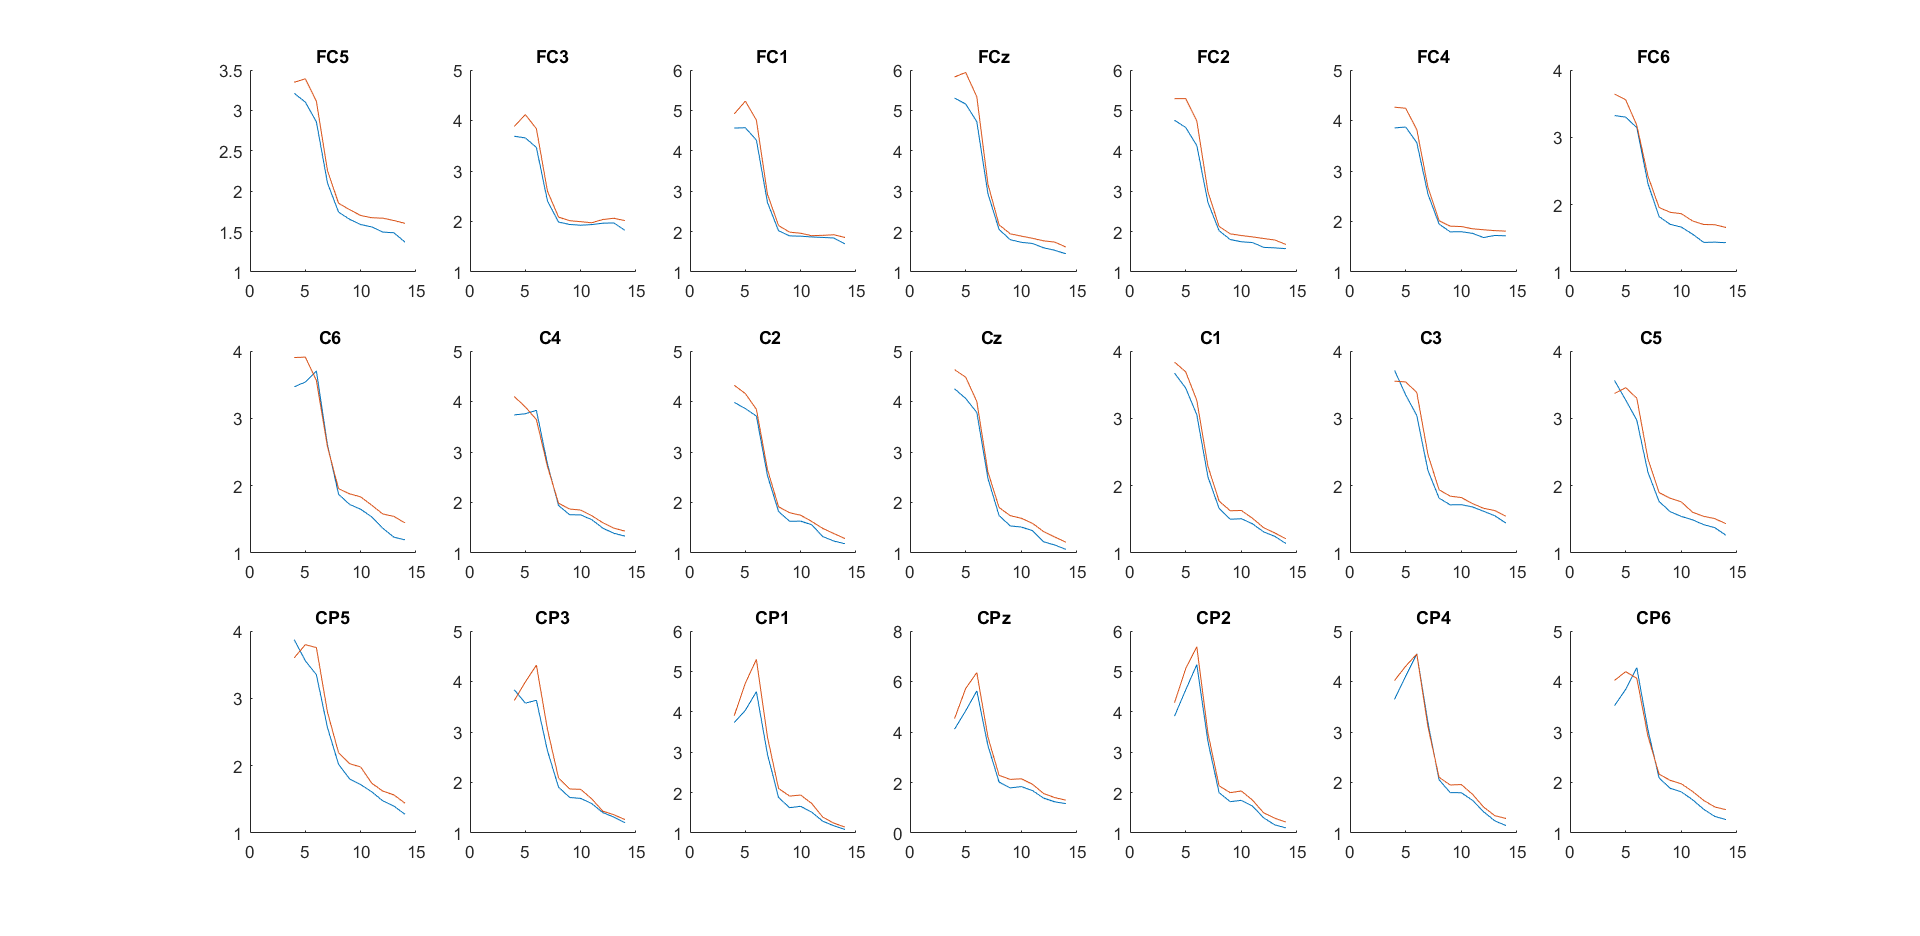
\includegraphics[width=1.0\textwidth]{distinction.png}
 \end{figure}

\end{frame}

\begin{frame}
  \frametitle{AWWW YEAH}

 \begin{figure}
  \centering
     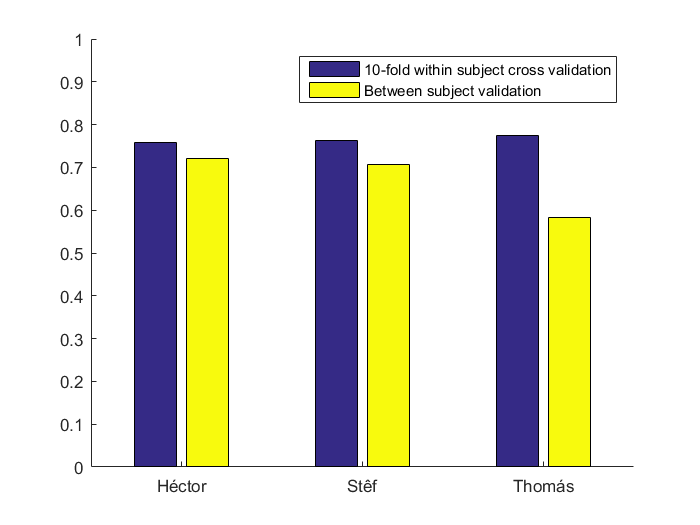
\includegraphics[width=0.7\textwidth]{bars.png}
 \end{figure}

\end{frame}

\section{Discussion}
\begin{frame}

\frametitle{Discussion}
  \begin{itemize}
   \item Adaptive approach produced sub-optimal results due to the necessity of unsupervised learning
   \item 
  \end{itemize}
\end{frame}



\begin{frame}

\frametitle{Take home message}
The adaptive approach did not work well but decent results were still obtained without training on the specific subject
\end{frame}

\end{document}
